\subsubsection{Financial Data Structures}

Four essential types of financial data
\begin{flushleft}
\begin{tabularx}{\textwidth}{X|X|p{13em}|X}
\hline
\rowcolor{gray!30}
Fundamental Data & Market Data & Analytics & Alternative Data \\
\hline
\xxx Assets 
\xxx Liabilities
\xxx Sales
\xxx Costs/Earnings
\xxx Macro Variables
\xxx $\cdots$
&
\xxx Price/Yield/IV
\xxx Volume
\xxx Dividend/Coupons
\xxx Open Interest
\xxx Quotes/Cancellations
\xxx Aggressor Side
\xxx $\cdots$
&
\xxx Analyst Recommendation
\xxx Credit Ratings
\xxx Earnings Expectations
\xxx News Sentiment
\xxx $\cdots$
&
\xxx Satellite/CCTV
\xxx Google Searches
\xxx Twitter/Chats
\xxx Metadata
\xxx $\cdots$ \\
\hline
\end{tabularx}
\end{flushleft}

\begin{remark} \hlt{Fundamental Data Characteristics}
\begin{enumerate}[label=\roman*.]
\setlength{\itemsep}{0pt}
\item Data published is indexed by last date included in report, which precedes date of release.
\item Data is often backfilled or re-instated, and data vendor may overwrite initial values with corrections.
\item Data is extremely regularised and low frequency.
\end{enumerate}
\end{remark}

\begin{remark} \hlt{Market Data Characteristics}
\begin{enumerate}[label=\roman*.]
\setlength{\itemsep}{0pt}
\item Raw feed contains unstructured information, such as FIX messages (allow full construction of trading book), or full collection of BWIC (bids wanted in competition) responses.
\item FIX data is not trivial to process, $\sim 10$TB generated on daily basis
\end{enumerate}
\end{remark}

\begin{remark} \hlt{Analytics Data Characteristics}
\begin{enumerate}[label=\roman*.]
\setlength{\itemsep}{0pt}
\item Derivative data as processed based on original source. Signal already extracted from the original source.
\item Costly, methodology used in production may be biased or opaque.
\end{enumerate}
\end{remark}

\begin{remark} \hlt{Alternative Data Characteristics}
\begin{enumerate}[label=\roman*.]
\setlength{\itemsep}{0pt}
\item Produced by individuals, business processes, and sensors.
\item Primary information that has not made it to other sources.
\item Cost and privacy concerns. May be useful if it annoys data infrastructure team.
\end{enumerate}
\end{remark}

\begin{figure}[H]
\centering
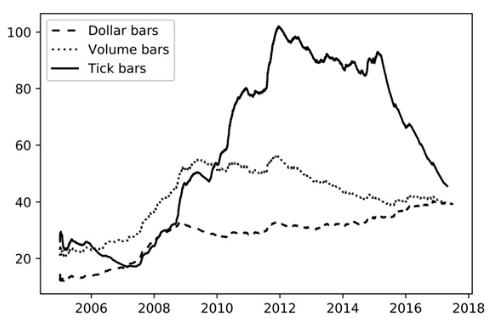
\includegraphics[scale=0.4]{/intro/standardbars}
\caption{Average daily frequency of tick, volume, and dollar bars}
\end{figure}

\begin{remark} \hlt{Standard BARS}\\
Method to transform a series of observations arriving at irregular frequency into a homogeneous series derived from regular sampling.
\begin{enumerate}[label=\roman*.]
\setlength{\itemsep}{0pt}
\item Time Bars: obtained by sampling information at fixed intervals. Information collected includes timestamp, volume-weighted average price (VWAP), open price, close price, high price, low price, volume etc.\\
To be avoided as markets do not process information at constant time interval. Time bars oversample information in low-activity periods and under-sample information in high-activity periods. Time bars exhibit poor statistical properties, i.e., serial correlation, heteroscedasticity, non-normality of returns.
\item Tick Bars: sample variables extracted each time a pre-defined number of transactions take place. Allows synchronisation of sampling with a proxy of information arrival.\\
Sampling as a function of trading activity creates returns closer to IID Normal (\cite{Thierry_Helyette_2000}). When constructing tick bars, to be aware of outliers, as many exchanges carry out auction at open and at close; order book accumulates bids and offers without matching. Order fragmentation introduces some arbitrariness in number of ticks. Matching engine protocols may split one fill into multiple artificial partial fills as a matter of operational convenience.
\item Volume Bars: samples every time a pre-defined amount of security's units that have been exchanged.\\
Achieves better statistical properties than sampling tick bars.\\
Convenient artefact for studying market microstructure theories.
\item Dollar Bars: samples an observation every time a pre-defined market value is exchanged. Used when the analysis involves significant price fluctuations. Robust against corporate actions such as splits, reverse splits, issuance of new shares, buying back existing shares.\\
Bar size could be dynamically adjusted as a function of free-floating market cap of a company or outstanding amount of issued debt.
\end{enumerate}
\end{remark}

\begin{remark} \hlt{Information-Driven Bars}\\
Method to sample more frequently when new (micro-structural) information arrives to the market.
\begin{enumerate}[label=\roman*.]
\setlength{\itemsep}{0pt}
\item Tick Imbalance Bars: sample bars whenever tick imbalance exceeds expectations. To determine tick index $T$ such that accumulation of signed ticks exceeds a given threshold.\\
Let $\{(p_t, v_t)\}_{t=1, \ldots, T}$ be sequence of ticks where $p_t$ and $v_t$ is the price and volume associated with tick $t$. Let tick rule define a sequence $\{b_t\}_{t=1, \ldots, T}$ where
\begin{align}
b_t = 
\begin{cases}
b_{t-1} \ \ \ \text{if } \Delta p_t = 0 \\
\frac{\abs{\Delta p_t}}{\Delta p_t} \ \ \text{if } \Delta p_t \neq 0
\end{cases} \nonumber
\end{align}
The tick imbalance at time $T$ is defined as 
\begin{equation}
\theta_T = \sum\limits_{t=1}^T b_t \nonumber
\end{equation}
Compute expected value of $\theta_T$ at beginning of the bar,
\begin{equation}
E_0[\theta_T] = E_0 [T](P[b_t = 1] - P[b_t = -1]) = E_0 [T](2P[b_t = 1] - 1) \nonumber
\end{equation}
where $E_0[T]$ is expected size of tick bar, $P[b_t = 1]$ and $P[b_t = -1]$ is unconditional probability that a tick is classified as a buy and sell. In practice, $E_0[T]$ and $(2P[b_t = 1] - 1)$ may be estimated as an exponentially weighted moving average of $T$ and $b_t$ values from prior bars.\\
Define the tick imbalance bar (TIB) as a $T^{*}$ contiguous subset of ticks such that
\begin{equation}
T^{*} = \arg \min_T \{ \abs{\theta_T} \geq E_0 [T] \ \vert \ 2 P[b_t = 1] - 1 \} \nonumber
\end{equation}
where the size of expected imbalance is implied by $\abs{2 P[b_t = 1] - 1}$.\\
When $\theta_T$ is more imbalanced than expected, a low $T$ will satisfy the conditions.\\
TIBs are produced more frequently under presence of informed trading (asymmetric information that triggers one-side trading). TIBs are buckets of trades containing equal amounts of information.
\item Volume/Dollar Imbalance Bars: sample bars when volume or dollar imbalances diverge from expectations.\\
First, define imbalance at time $T$ as
\begin{equation}
\theta_T = \sum\limits_{t=1}^T b_t v_t \nonumber
\end{equation}
where $v_t$ may represent ether number of securities traded (VIB) or dollar amount traded (DIB).\\
The expected value of $\theta_T$ at the beginning of the bar is then computed as
\begin{align}
E_0[\theta_T] &= E_0 \left[ \sum\limits_{t \vert b_t = 1}^T v_t \right] - E_0 \left[ \sum\limits_{t \vert b_t = -1}^T v_t \right] \nonumber \\
&= E_0[T] (P[b_t = 1]E_0[v_t \vert b_t = 1] - P[b_t = -1]E_0[v_t \vert b_t = -1]) \nonumber \\
&= E_0[T] (v^+ - v^-) \nonumber
\end{align}
where the initial expectation of $v_t$ is decomposed into component contributed by buys and sells. Then
\begin{equation}
E_0[\theta_T] = E_0[T] (2v^+ - E_0 [v_t]) \nonumber
\end{equation}
In practice, $E_0[T]$ and $(2v^+ - E_0 [v_t])$ may be estimated as exponentially weighted moving average of $T$ and $b_t v_t$ values from prior bars. Next, define VIB or DIB as a $T^*$-contiguous subset of ticks such that
\begin{equation}
T^* = \arg \min_T \{ \abs{\theta_T} \geq E_0[T] \ \vert \ 2v^+ - E_0[v_t] \} \nonumber
\end{equation}
where the size of expected imbalance is implied by $\abs{2v^+ - E_0[v_t]}$.\\
When $\theta_T$ is more imbalanced then expected, a low $T$ will satisfy the conditions.\\
VIB and DIB addresses concerns on tick fragmentation and outliers, and also addresses the issues of corporate actions, as the bar size is adjusted dynamically.
\item Tick Runs Bars: sample bars when the sequence of buys in overall volume diverges from expectations. For the case when large traders sweep order book, use iceberg orders, or slice parent orders into multiple children, all leaving a trace of runs in the $\{b_t\}_{t = 1, \ldots, T}$ sequence. Define length of current run as
\begin{equation}
\theta_T = \max \left\{ \sum\limits_{t \vert b_t = 1}^T b_t - \sum\limits_{t \vert b_t = -1}^T b_t  \right\} \nonumber
\end{equation}
The expected value of $\theta_T$ at beginning of bar is computed as
\begin{equation}
E_0[\theta_T] = E_0[T] \max \{P[b_t = 1], 1 - P[b_t = 1] \} \nonumber
\end{equation}
In practice, $E_0[T]$ and $P[b_t = 1]$ may be estimated as exponentially weighted moving average of $T$ and proportion of buy ticks from prior bars. Next, define TRB as $T^*$-contiguous subset of ticks such that
\begin{equation}
T^* = \arg \min_T \{ \theta_T \geq E_0[T] \max \{P[b_t = 1], 1 - P[b_t = 1] \} \} \nonumber
\end{equation}
where the expected count of ticks from runs is implied by $\max \{P[b_t = 1], 1 - P[b_t = 1] \}$.\\
When $\theta_T$ exhibits more runs than expected, a low $T$ will satisfy these conditions.\\
Instead of measuring length of longest sequence, count number of ticks of each side without offsetting.
\item Volume/Dollar Runs Bars: sample bars when volume or dollars traded by one side exceed expectation for a bar. First, define volume or dollars associated with a run as
\begin{equation}
\theta_T = \max \left\{ \sum\limits_{t \vert b_t = 1}^T b_t v_t - \sum\limits_{t \vert b_t = -1}^T b_t v_t \right\} \nonumber
\end{equation}
where $v_t$ may either represent volume (VRB) or dollar amount exchanged (DRB). The expected value of $\theta_T$ at beginning of the bar is then
\begin{align}
E_0 [\theta_T] = E_0[T] \max \{ P[b_t = 1]E_0[v_t \vert b_t = 1], (1 - P[b_t = 1]) E_0[v_t \vert b_t = -1] \} \nonumber
\end{align}
In practice, $E_0[T], P[b_t = 1], E_0[v_t \vert b_t = 1], E_0[v_t \vert b_t = -1]$ may be estimated as exponentially weighted moving average of $T$, proportion of buy ticks, buy volumes, and sell volumes from prior bars. Next, define a volume runs bar (VR) as $T^*$-contiguous subset of ticks such that
\begin{equation}
T^* = \arg \min_T \{ \theta_T \geq E_0[T] \max \{P[b_t = 1]E_0[v_t \vert b_t = 1], (1 - P[b_t = 1]) E_0[v_t \vert b_t = -1] \} \} \nonumber
\end{equation}
expected volume from runs is implied by $\max \{P[b_t = 1]E_0[v_t \vert b_t = 1], (1 - P[b_t = 1]) E_0[v_t \vert b_t = -1] \} \}$.\\
When $\theta_T$ exhibits more runs than expected, volume from runs is greater than expected, a low $T$ will satisfy these conditions.
\end{enumerate}
\end{remark}

\begin{definition} \hlt{Multi-Product Series: ETF Trick}\\
To model a basket of securities as if it was a single cash product. To transform any complex multi-product dataset into a single dataset that resembles a total return ETF.
\end{definition}

\begin{method} \hlt{ETF Trick}\\
Produce a time series that reflects the value of $\$1$ invested. Changes in the series will reflect changes in PnL, series will be strictly positive, and implementation shortfall will be taken into account. The bars contain:
\begin{enumerate}[label=\roman*.]
\setlength{\itemsep}{0pt}
\item Raw open price of instrument $i = 1, \ldots, I$ at bar $t = 1, \ldots, T$: $o_{i,t}$
\item Raw close price of instrument $i = 1, \ldots, I$ at bar $t = 1, \ldots, T$: $p_{i,t}$
\item USD value of one point of instrument $i = 1, \ldots, I$ at bar $t = 1, \ldots, T$: $\varphi_{i,t}$. This includes forex rate.
\item Volume of instrument $i = 1, \ldots, I$ at bar $t = 1, \ldots, T$: $v_{i,t}$
\item Carry, dividend, or coupon paid by instrument $i$ at bar $t$: $d_{i,t}$. Variable can also be used to charge margin costs or costs of funding.
\end{enumerate}
All instruments $i = 1, \ldots, I$ were tradable at bar $t = 1, \ldots, T$. Even if some instruments were not tradable over entirety of time interval $[t-1, t]$, at least they were tradable at times $t-1$ and $t$.\\
For basket of securities with allocation vector $\omega_t$ rebalanced (or rolled) on bars $B \subseteq \{1, \ldots, T \}$, the $\$1$ investment value $\{K_t\}$ is derived as 
\begin{align}
h_{i,t} &= 
\begin{cases}
\frac{\omega_{i,t} K_t}{o_{i, i+1} \varphi_{i,t} \sum\limits_{i=1}^I \abs{\omega_{i,t}}} \ \ \ \text{if } t \in B \\
h_{i, t - 1} \ \ \ \ \ \ \ \ \ \ \ \ \ \ \ \ \text{otherwise}
\end{cases} \nonumber \\
\delta_{i,t} &=
\begin{cases}
p_{i,t} - o_{i,t} \ \ \ \text{if } (t-1) \in B \\
\Delta p_{i,t} \ \ \ \ \ \ \ \ \ \ \ \ \ \ \ \ \ \text{otherwise}
\end{cases} \nonumber \\
K_t &= K_{t-1} + \sum\limits_{i=1}^I h_{i, t-1} \varphi_{i,t} (\delta_{i,t} + d_{i,t}) \nonumber
\end{align}
where $K_0 = 1$ is the initial AUM. Variable $h_{i,t}$ is the holdings of instrument $i$ at time $t$, $\delta_{i,t}$ is change of market value between $t-1$ and $t$ for instrument $i$. Note profits or losses are being reinvested whenever $t \in B$, hence preventing negative prices. Dividends $d_{i,t}$ are already embedded in $K_t$.\\
The purpose of $\omega_{i,t} \left( \sum_{i=1}^I \abs{\omega_{i,t}} \right)^{-1}$ is to de-lever the allocations.\\
Let $\tau_i$ be transaction cost associated with trading $\$1$ of the instrument. Three additional variables that the strategy needs to know for every observed bar $t$ are:
\begin{enumerate}[label=\roman*.]
\setlength{\itemsep}{0pt}
\item Rebalance Costs: variable cost $\{c_t\}$ associated with allocation rebalance is
\begin{equation}
c_t = \sum\limits_{i=1}^I (\abs{h_{i, t-1}}p_{i,t} + \abs{h_{i,t}} o_{i, t+1}) \varphi_{i,t} \tau_{i} \ \ \ \forall t \in B \nonumber
\end{equation}
Note $c_t$ is not embedded in $K_t$, as shorting will generate fictitious proceeds when allocation is rebalanced.\\
In code, $\{c_t\}$ is treated as a (negative) dividend.
\item Bid-Ask Spread: the cost $\{ \tilde{c}_t \}$ of buying or selling one unit of this ETF,
\begin{equation}
\tilde{c}_t = \sum\limits_{i=1}^I \abs{h_{i, t-1}}p_{i, t} \varphi_{i,t} \tau_i \nonumber
\end{equation}
When a unit is bought or sold, strategy must charge this cost $\tilde{c}_t$.
\item Volume: volume traded $\{v_t \}$ is determined by least active member in the basket. Let $v_{i,t}$ be volume traded by instrument $i$ over bar $t$. The number of tradable basket units is
\begin{equation}
v_t = \min_i \left\{ \frac{v_{i,t}}{\abs{h_{i, t-1}}} \right\} \nonumber
\end{equation}
Transaction costs functions may not be linear, and can be simulated by the strategy.
\end{enumerate}
\end{method}